\section{Embedded Peripherals}
\subsection{Timers and Event Counters}
\subsubsection{Timer Structure}
A Binary Counter Driven by a Periodic Signal.It is possible to cascade multiple counters\\
\vspace{1cm}
\begin{minipage}{9cm}
	\begin{itemize}
		\item Mux -> Clock Source selector
		\item Prescaler -> Clock frequency divider
		\item Counter -> n-bit binary counter
		\item Comparator -> compares Counter Output with Compare Register
	\end{itemize}
\end{minipage}
\begin{minipage}{10cm}
	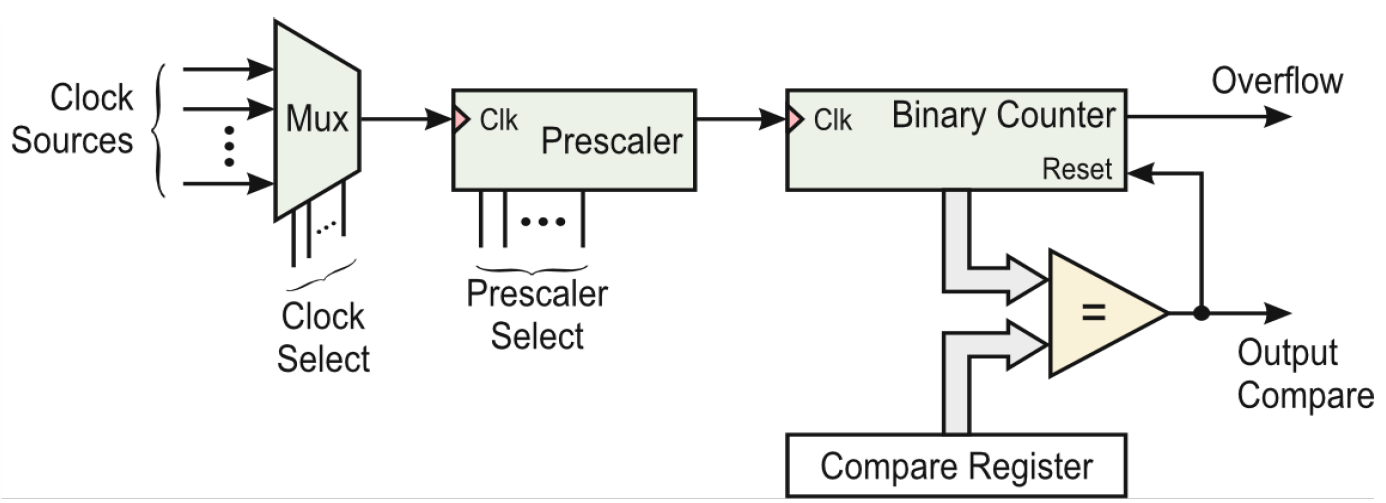
\includegraphics[width=10cm]{images/timerstructure.png} 
\end{minipage}
\begin{multicols}{2}
	\subsubsection{Interval Timer vs Event Counter}
	\begin{itemize}
		\item \textbf{Interval Timer}
		\subitem Measures the time elapsed after k clock cycles
		\item \textbf{Event Counter}
		\subitem Counts the occurrence of k external events
	\end{itemize}
	
	\subsubsection{Timer Application}
	\begin{itemize}
		\item Watchdog Timers (WDT)
		\item Realtime Clocks (RTC)
		\item Baud Rate Generator (BRG)
		\item Pulse-Width Modultation (PWM)
	\end{itemize}
\end{multicols}

\textbf{Signature Timer Application 7.4.3 \embsys{336}}\newline
\begin{tabular}{p{5cm} p{15cm}}
	\textbf{Watchdog Timer } &
    Monitor Events within an expiration intervals\newline
	 If WDT expires before the event occurs, a default action is executed\newline
	 If the event occurs within the defined interval, cancel and restart WDT\newline
	 In MSP430 the WDT is 16-Bit (MaxCount: $2^{16}=32'768$) \newline
	 and configure over Register WDTTMSEL\\
     
	\textbf{Realtime Clocks} &
    32-bit Timer with selectable Clock-Source\newline
    Can be used as calendar or counter (H.Min.Sec)\newline
    The accuracy depeands greatly on the used Cristal\\
    
	\textbf{Baud Rate Generator} &
     $ \text{baude Rate}=\dfrac{f_{clk}}{PS \cdot TopCount} $\newline
     PS=Prescaler Value \quad TC= Compare Value\newline
     Directly impacts Bit Time on serial communication\\
     
	\textbf{Pulse-Width Modulation} &
    Produces a Signal whose duty cycle is controlled by the MCU \newline
    $ \text{duty cycle}=\dfrac{t_{high}}{T} $\\
\end{tabular}


\clearpage
\pagebreak